\documentclass[a4paper, oneside]{article}
\usepackage[T1]{fontenc}
\usepackage[utf8]{inputenc}
\usepackage[english]{babel}
\usepackage{frontespizio}
\usepackage{float}
\usepackage{graphicx}
\usepackage{listings}
\usepackage{scrextend}
\usepackage[margin=1.2in]{geometry}
\usepackage[font=small,labelfont=bf]{caption}
\usepackage{url}
\usepackage{verbatim}

\begin{document}
\selectlanguage{english}
\baselineskip 13pt

% ---- FRONTESPIZIO ----- 
\begin{frontespizio} 
 \Preambolo{\renewcommand{\frontpretitlefont}{\fontsize{15}{12}\scshape}}
\Istituzione {University of Pisa}
\Divisione {Scuola di Ingegneria}
\Corso [Laurea]{Artificial Intelligence and Data Engineering}
\Annoaccademico {2019--2020}
\Titolo {Moviegram documentation}
\Filigrana [height=4cm,before=0.28,after=1]{./images/stemma_unipi.png}
\Rientro {1cm}
\Candidato {Alice Nannini}
\Candidato {Giacomo Mantovani}
\Candidato {Marco Parola}
\Candidato {Stefano Poleggi}
\Relatore {Prof. Pietro Ducange}
 \Punteggiatura {}
\end{frontespizio}

\clearpage

% ----- INDICE -----
	\tableofcontents\thispagestyle{empty}
	\clearpage


\section{Introduction}\pagenumbering{arabic}
The \textbf{Moviegram} application offers a search and information service in the field of cinema. When the application starts, the system requires authentication to use the service.
The logged-in user can perform a search by entering the first characters of a movie title in the search bar, obtaining a list of 10 movies in the database. After that you can select one of the proposed titles or carry out a more in-depth search, adding characters.
Selecting a row, the system allows you to view more information in the right section, including cover, title, director and ratings.
The user can leave a mark from 1 to 5 for the selected movie.
There is also a module for the system administrator: when he logs in, he's redirected to a different activity than the user's one. In this page, he can view some statistics linked to the movies and the searches carried out by the users of the application, such as the ranking of 10 most voted films or the 10 most sought after films.
Moreover, the system admin can add new movies to the application database or delete those already present, by searching by title.

\begin{figure}[h]
\centering
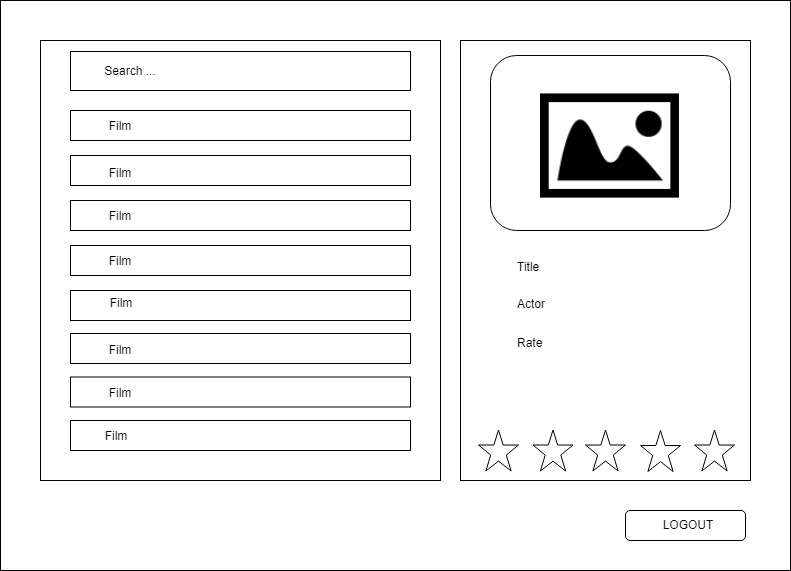
\includegraphics[width=\textwidth]{./images/diagrams/UserMockup} 
\caption{User Mockup}
\label{fig:mockup}
\end{figure}

\begin{figure}[h]
\centering
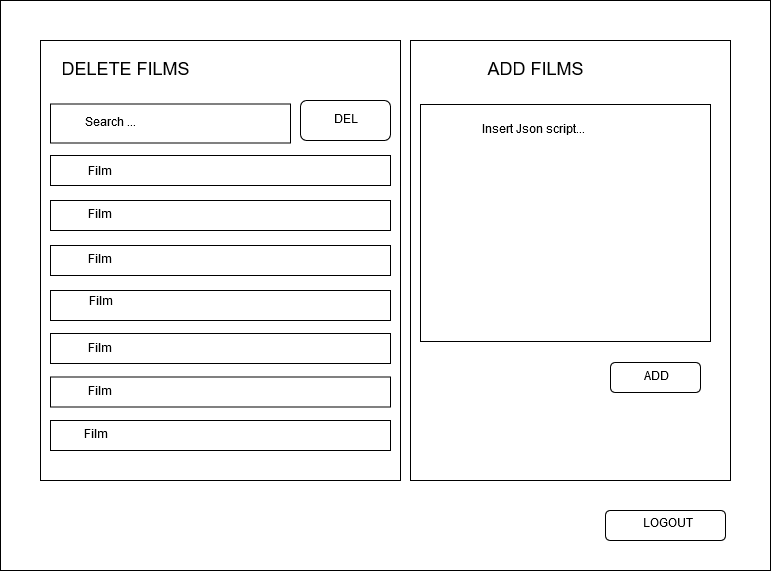
\includegraphics[width=\textwidth]{./images/diagrams/admin_activity}
\caption{Admin Mockup}
\label{fig:mockup_admin}
\end{figure}

\clearpage

\section{Analysis and workflow}

% ----- REQUIREMENTS -----
\subsection{Requirements}

\subsubsection{Functional requirement}
The system has to allow the user to carry out basic functions such as:
\begin{itemize}
\item To sign up into the system.
\item To login to the system.
\item To search for a movie.
\item To vote a movie.
\item To view a list of the top rated movies, both in general and filtered by a selected country.
\item To view a list of the top production houses.
\item To view the top countries in making movies, filtered by a selected year.
\item To view the most active users in the application, i.e. the users that have given most votes.
\end{itemize}
\vspace{2mm}
The system has to allow the administrator to carry out basic functions such as:
\begin{itemize}
\item To login to the system.
\item To add a movie.
\item To delete a movie.
\end{itemize}
\vspace{2mm}

\subsubsection{Non-functional requirements}
\begin{itemize}
\item Usability, ease of use and intuitiveness of the application by the user.
\item Availability, with the service guaranteed h24, using replicas.
\item The system should provide access to the database with a few seconds of latency.
\item Eventual consistency.
\end{itemize}

\clearpage

% ----- USE CASES -----
\subsection{Use Cases}

\textbf{Actors}
\begin{itemize}
\item{User: this actor represents a user of the application}
\item{Admin: this actor represents the administrator of the application}
\end{itemize}

\subsubsection{Use Cases Description}
\begin{table}[h]
\centering
\begin{tabular}{p{0.16\textwidth}p{0.2\textwidth}lp{0.5\textwidth}}

% ----- USE CASES TABLE -----
\hline
\textbf{Event} & \textbf{UseCase} & \textbf{Actor(s)} & \textbf{Description}\\ \hline
Log in, Log out & Login,  Logout & Admin, User & The user logs in/out the application.\\ \hline

Sign up & Sign up & User & The user sign in the application.\\ \hline

Scan data to perform query & Browse Films, Find By parameter & User, Admin & This use cases are involved in all the operations related to retrieve data from db, moreover it is possible to pass a parameter to the find function. \\ \hline

Set searching parameter &  By country, By title, By year & User, Admin & Use case related to selecting a parameter to pass to other use cases.\\ \hline

Search movies & Search Film & User, Admin & Use case related to the functionality of searching some movies.\\ \hline

Display all the movies & Display Films & User, Admin & The user chooses that he wants to view the list of Films. The system browses the data on the db (using browse and find use cases) and returns them on the interface.\\ \hline

Display the movies ranking & View Top Rated Films & User, Admin & Use case related to the functionality of searching the movies, sorted by the rate. \\ \hline

Display the production houses ranking & View Top Productions & User, Admin & Use case related to the functionality of searching the production houses, sorted by the number of movies produced. \\ \hline

Display the ranking of the countries & View Top Rated  By Year And Country & User, Admin & Use case related to the functionality of searching the countries, sorted by the number of movies produced, given a year. \\ \hline

Display most active users & View Top Active Users & Admin & Use case related to the functionality of searching the users, sorted by the number of votes given.\\ \hline

Add a film & Add Film & Admin & The admin submits the Film information. The system updates the db and the interface.\\ \hline

Delete a film & Delete Film & Admin & The admin selects the film and submits the delete. The system updates the db and the interface.\\ \hline

View the film informations & Display Film Informations & User, Admin & The user selects the film. The system shows the film informations on the interface.\\ \hline

Vote a film & Add Vote & User, Admin & The user submits the vote on a selected film. The system updates the db and the interface.\\ \hline

\end{tabular}
\end{table}

\begin{minipage}{\linewidth}
\begin{center}
\vspace{8mm}
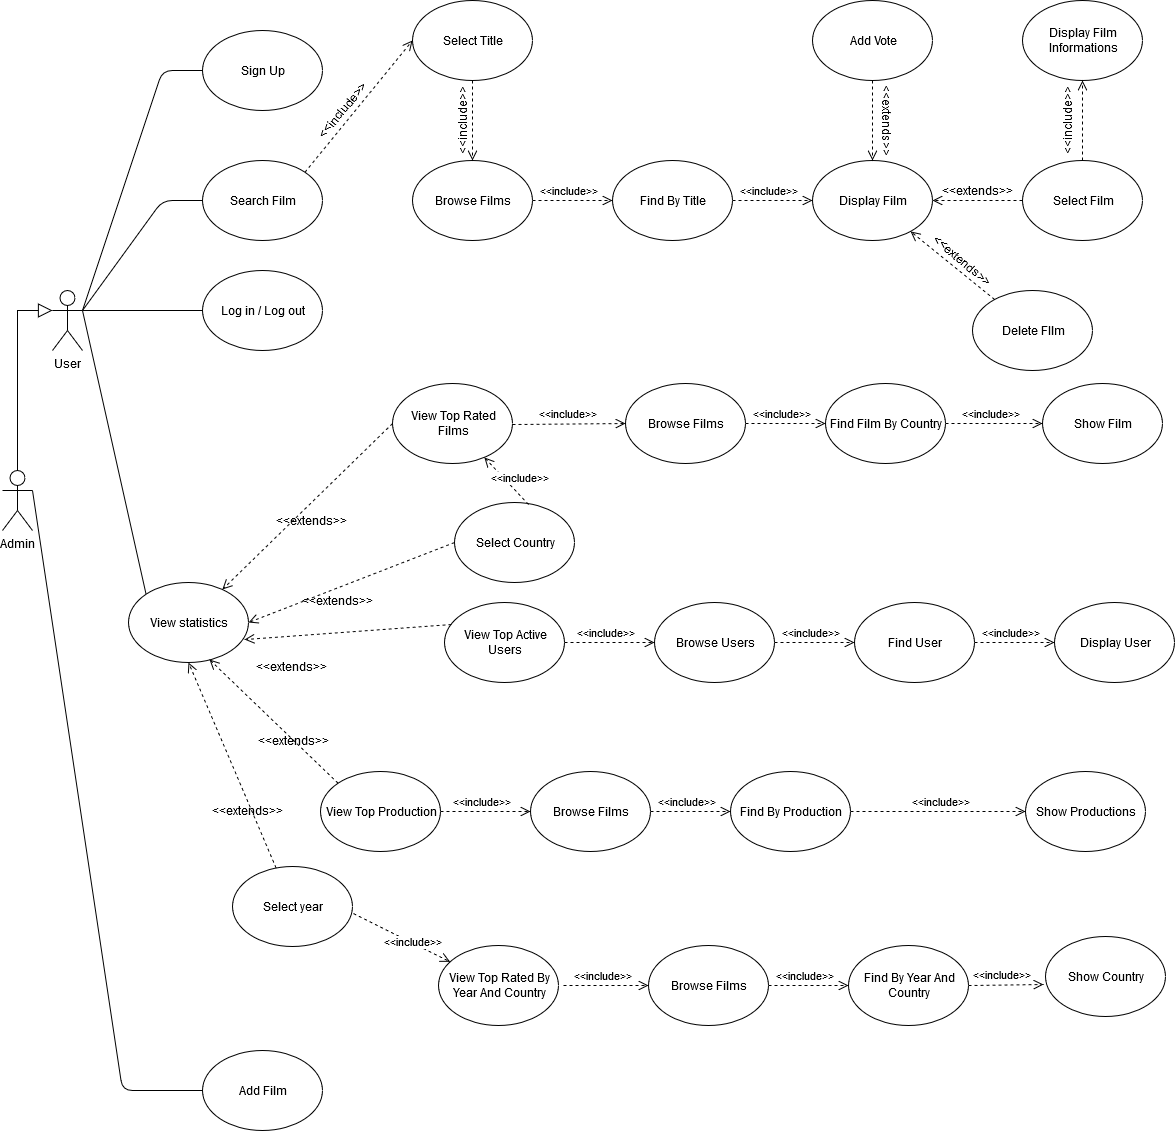
\includegraphics[ width=0.7\textheight]{./images/diagrams/UseCase.png} 
\captionof{figure}{Use cases diagram}
\vspace{3mm}
\end{center}
\end{minipage}


\clearpage


\subsection{Analysis of entities}
This diagram represents the main entities of the application and the relations between them.
\begin{minipage}{\linewidth}
\begin{center}
\vspace{4mm}
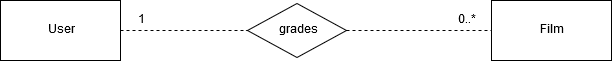
\includegraphics[width = 0.7\textwidth]{./images/diagrams/Analysisuml} 
\vspace{2mm}
\captionof{figure}{UML analysis diagram}
\label{fig:useCases}
\end{center}
\end{minipage}



\clearpage
% ----- DESIGN -----
\section{Design}

\subsection{Database Choice}
After the analysis phase, which has been carried out so far, we start with the design of the \textbf{Moviegram} application. We decide to use MongoDB as data support. Its document-based structure is very useful for the large amount of data that we need to maintain and access, as well as its high scalability, qualities that we do not find in a relational database. Thanks to the help of indexes, we can make very fast queries, while thanks to replicas we can guarantee the data availability.


% ----- ACHITECTURE -----
\subsection{Software architecture}
The application is designed over 2 different layers, see figure \ref{fig:architecture_diagram}:
\begin{itemize}
\item Front-end
\item Back-end
\end{itemize}
\vspace{5mm}
\begin{minipage}{\linewidth}
\begin{center}
\vspace{1mm}
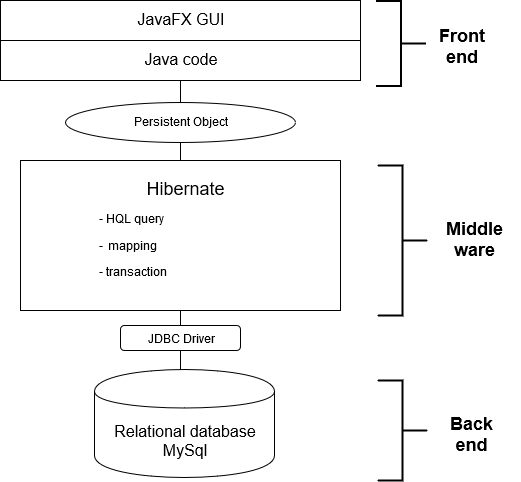
\includegraphics[height = 100mm]{./images/diagrams/architecture_diagram.png} 
\vspace{6mm}
\captionof{figure}{Software architecture diagram\\}
\label{fig:architecture_diagram}
\end{center}
\end{minipage}
\vspace{7mm}
\clearpage


\subsection{Prepare connection to guarantee Availability}
In order to guarantee a high level of availability, we give back the control to application after the write on the primary server, without waiting the update of all replicas.
As said previous, this choice guarantee a good perfomance in term of speed, but decrease the part related to consistency, it could happen that a user reads some "old" data from a replica, in case of primary server failure.
\begin{verbatim}
     mongoClient = MongoClients.create(
        MongoClientSettings.builder()
                .applyToClusterSettings(builder ->
                        builder.hosts(Arrays.asList(new ServerAddress(ip0, port0),
                                                    new ServerAddress(ip1, port1),
                                                    new ServerAddress(ip2, port2))))
                         .writeConcern(new WriteConcern().ACKNOWLEDGED)
                .build());
\end{verbatim}
% ----- RETRIEVE DATA -----
\subsection{Populating the database}
The dataset used in the \textbf{Moviegram} application was created by scraping the Open Movie Database, using their API (\url{http://www.omdbapi.com/}). Given a movie title, this API returns all the information in the OMDb about that movie. Before started building up the dataset using the API, it was necessary to obtain a list of movie titles, to be passed to the API; the list of titles was built up using different web pages as sources:
\begin{itemize}
\item a page of Wikipedia was scraped
\item the pages referring to each year from 2007 to 2021 on the site \url{https://www.wildaboutmovies.com/} were scraped
\item a csv file in the GitHub repository \url{https://github.com/fivethirtyeight/data} was used
\end{itemize}
Once the titles’ list was ready, the only thing left to do was to obtain the key requested by the OMDb API to download the films’ information. Each key provided by the database allows a user to download 1000 film’s information per day. Once the movies’ list and the keys were ready, we could start to use our scraping application.\\

\begin{minipage}{\linewidth}
\begin{center}
\vspace{1mm}
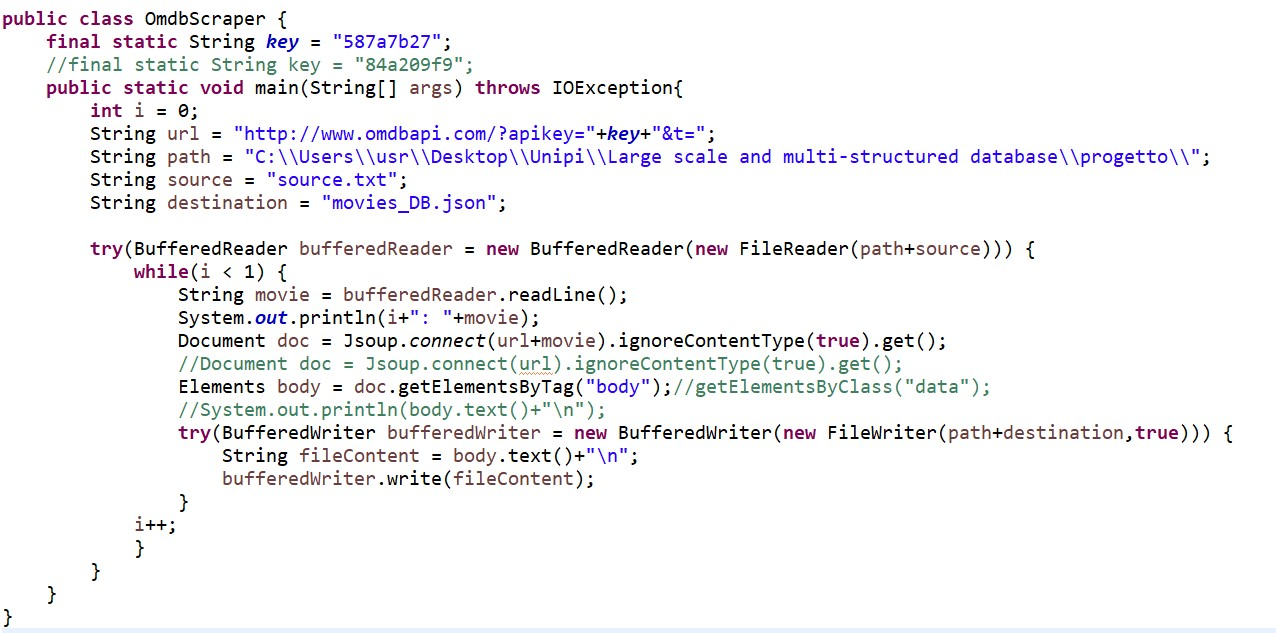
\includegraphics[height = 80mm]{./images/screens/OMDBScraperScreen.jpg} 
\vspace{6mm}
\captionof{figure}{Java class of OMDBScraper\\}
\label{fig:OMDBScraper}
\vspace{2mm}
\end{center}
\end{minipage}
Using our “OmdbScraper” application, we managed to obtain the collection of movies’ information in a JSON format.\\ The format of our JSON elements are the following:

\begin{minipage}{\linewidth}
\begin{center}
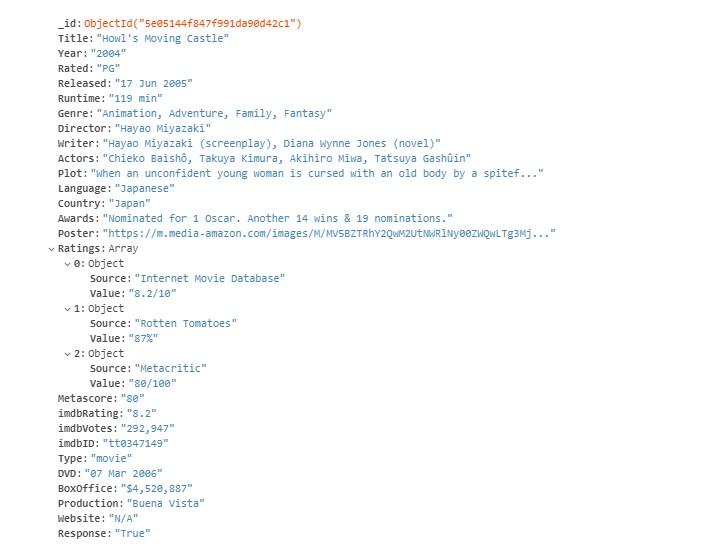
\includegraphics[height = 80mm]{./images/screens/elementJSONExample.jpg} 
\vspace{2mm}
\captionof{figure}{Example of JSON document\\}
\label{fig:elementJSONExample}
\vspace{5mm}
\end{center}
\end{minipage}
We integrated our movies dataset with a plot dataset, found on \url{kaggle.com} (wiki\_plot). In order to do so, we searched for matching between the plot’s movie title and the movie title in our collection; once the matching was found, the plot field in the original element was replaced with the data presents in the plot dataset.\\

% ----- COLLECTIONS -----
\subsubsection{Collections}
At the end we modeled all the entities in two collections: \textit{moviesCollection} and \textit{usersCollection}.\\
The first one store all the information related to each movie, also the following entities: actors, production houses, writers and directors. An example is shown in figure \ref{fig:elementJSONExample}.\\
The second collection stores all information related to the users (name, username, password, and country), in this case we store also the entity Vote, inserting each Vote in an array. We decide to store the votes that a user give to a movies in an array in usersCollections instead to store the votes that a movie received in the moviesCollection, because in the application we are interested to retrieve the votes given by the logged user.
\begin{figure}[H]
\centering
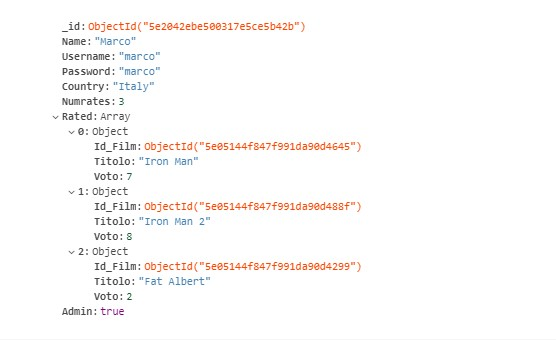
\includegraphics[width=0.57\textwidth]{./images/screens/userCollection} 
\caption{Example of document of collection of user.}
\label{fig:admin1}
\end{figure}

\subsubsection{Data type transformation}
Moreover, we managed some data types because, scraping the OpenMovie platform, we'd obtained every field in a string format, but to compute the analytics operations described in the functional requirements section, we need to have some fields in a number format. We ran the following javascript code on the mongo shell, to perform the conversion:
\vspace{2mm}
% ----- android wearable module -----
\begin{lstlisting}[language=Java,  basicstyle=\footnotesize]
	db.collection.find().foerEach( function(x){
		x.ratingImdb = parseFloat( x.imdbRating);
		db.collection.save(x);
	});
\end{lstlisting}
\vspace{5mm}


% ----- INDEXES -----
\subsection{MongoDb indexes}
\subsubsection{Index 1}
In order to speeding up the operation that displays the top rated movies, we introduce an index on the field 'Ratings', because also the mongo shell suggests to introduced it, when we execute the query.
\begin{figure}[H]
\centering
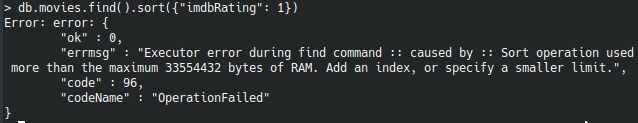
\includegraphics[width=0.6\textwidth]{./images/screens/errorSize} 
\caption{Mongodb error.}
\label{fig:admin1}
\end{figure}
The following snippet of code shows the query and its result in term of performance, limiting the number of records (8000). The query takes 61 milliseconds to be executed, without introducing any index.
\begin{verbatim}
     db.movies.find().sort({"imdbRating" : 1}).explain("executionStats");
\end{verbatim}
\begin{figure}[H]
\centering
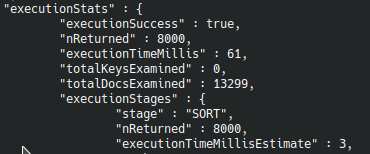
\includegraphics[width=0.4\textwidth]{./images/screens/timeNoIndex} 
\caption{Performance before inserting the index.}
\label{fig:admin1}
\end{figure}
So we introduce an index on imdbRating field and we execute again the query to evaluate the performance.
\begin{figure}[H]
\centering
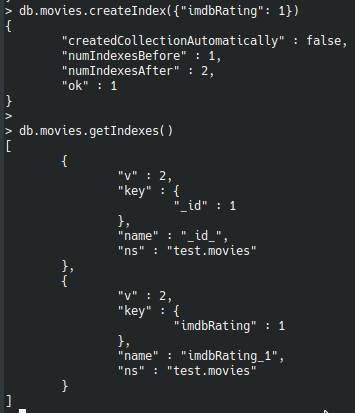
\includegraphics[width=0.4\textwidth]{./images/screens/createIndex} 
\caption{Create index.}
\label{fig:admin1}
\end{figure}
\begin{figure}[H]
\centering
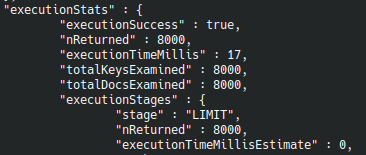
\includegraphics[width=0.45\textwidth]{./images/screens/timeIndex} 
\caption{Performance after inserting the index.}
\label{fig:admin1}
\end{figure}
We can observe that the execution time decrease to 17 milliseconds.
However this index decrease the performance of the operation that displays the top movies selecting a country, but we expect the previous operation to be compute more frequently.

\subsubsection{Index 2}
This index is related to the users collection. This collection is indexed using 'Numrates', a counter for the number of rates that a user has given.
This index will improve the performance of the operation that returns the ranking of the most active users on the plattform.
\begin{verbatim}
     db.users.createIndex({"Numrates" : -1 });
\end{verbatim}
It isn't shown the analysis of the performance as in the previous index, because the data of the user are built to test the application and they aren't real.

% ----- ANALYTICS -----
\subsection{Analytics and statistics}
\subsubsection{View the top production houses}
This analytic is performed to display the production houses that produced the most films. To do so, we make an aggregation pipeline to recover from our database the information about the production houses’ production. \\
The first thing to do is to filter out the document with a “N/A” value in the production field; done that, we aggregate on Production (production houses) summing every film made by that specific company; as a last thing to do, we order the resulting documents in ascending order.\\
View top production.Aggregate per production summing up, excluding “N/A” and sorting.
\begin{verbatim}
   db.Films.aggregate([
       {$match:{  Production: {$ne: “N/A”}}},
       {$group:{ _id: “$Production”, NFilm: {$sum: 1}}},
       {$sort:{NFilm: -1}}
   ]);
\end{verbatim}


\subsubsection{View top 10 country of production, once selected a year}
In that case, we let the user choose the year for which compute the aggregation. The users’ year choose is passed to the java function that will produce the aggregation. In our example we selected the year 2005.\\
The first thing we do is selecting only the records for the chosen year, this is done with the \$match phase. The second thing we do is grouping per “\$Country” and summing up all the document for that country; the last thing we do is the sorting in ascendant order relying on the NFilms field.
\begin{verbatim}
   db.Films.aggregate([
       {$match:{ Year : "2005"}},
       {$group:{ _id: “$Country”, NFilms:{ $sum: sum:1}}},
       {$sort:{ NFilms:-1}}
   ]);
\end{verbatim}

\clearpage

% ----- IMPLEMENTATION -----
\section{Implementation}
\subsection{Used technologies}
The application is developed in java programming language, version 11.0.4, and in JavaFX system to create the GUI, version 11, so it should run on each platform in which JVM is installed, but the application is tested and guardantee on Ubuntu 16 and Window OS. Moreover Maven is used  to build and mantain the project, version 3.8.0. \\
The java driver for mongo manage the comunication between client application layer and mongo backend layer, version 3.11.2.\\ 
For the backend layer it is used MongoDB, version 4.2.\\
So this application is tested using these technologies, considering these particular versions: for other versions the correct execution isn't guaranteed .\\

\subsection{Replica setup}
The following code shows how it is realized the architecture in which 3 mongo server are running in back end layer:
\vspace{2mm}
% ----- android wearable module -----
\begin{lstlisting}[language=Java,  basicstyle=\footnotesize]
# ----- PREPARAZIONE CARTELLE PER LOG E PER I DB -----
sudo mkdir -p /srv/mongodb/rs0-0 /srv/mongodb/rs0-1 /srv/mongodb/rs0-2
sudo mkdir -p /var/log/mongodb/rs0-0 /var/log/mongodb/rs0-1 /var/log/mongodb/rs0-2

# ----- RUN 3 ISTANCES OF MONGOD -----
sudo mongod --port 27017 --dbpath /srv/mongodb/rs0-0 --replSet rs0 --oplogSize 128
--logpath /var/log/mongodb/rs0-0/server.log --fork
sudo mongod --port 27018 --dbpath /srv/mongodb/rs0-1 --replSet rs0 --oplogSize 128 
--logpath /var/log/mongodb/rs0-1/server.log --fork
sudo mongod --port 27019 --dbpath /srv/mongodb/rs0-2 --replSet rs0 --oplogSize 128 
--logpath /var/log/mongodb/rs0-2/server.log --fork

# ----- CHECK LISTENING PROCESS -----
netstat -tulpn

# ----- CONNECT TO PRIMARY MONGOD ISTANCE -----
mongo --port 27017

/* JS SCRIPT */
var rsconf = {
    _id: "rs0",
    members: [
                {_id: 0,  host: "127.0.0.1:27017"},
                {_id: 1,  host: "127.0.0.1:27018"},
                {_id: 2,  host: "127.0.0.1:27019"}
            ]
};
rs.initiate( rsconf );
rs.conf();
rs.status();

# ----- KILL PROCESS USING PORT -----
sudo fuser -k 27017/tcp
sudo fuser -k 27018/tcp
sudo fuser -k 27019/tcp

# ----- ELIMINA CARTELLE ------
sudo rm -r /srv/mongodb/rs0-0 /srv/mongodb/rs0-1 /srv/mongodb/rs0-2
sudo rm -r /var/log/mongodb/rs0-0 /var/log/mongodb/rs0-1 /var/log/mongodb/rs0-2

\end{lstlisting}
\vspace{5mm}
\subsection{Java class description}
\subsubsection{Declaration of class Film}
The following java-code shows a declaration of the class Film.
\vspace{2mm}
% ----- android wearable module -----
\begin{lstlisting}[language=Java,  basicstyle=\footnotesize]
public class Film {
	private String id;
	private SimpleStringProperty title;
	private String director;
	private String production;
	private String poster;
	private int year;
	private Double rating;
	private int votes;
	

	public Film(String _id, String title, String director,
	 String production,	String poster, String year, String rating,
	  String votes) {
		
		id = _id;
		if (!rating.equals("N/A")) {
			this.rating = Double.parseDouble(rating);
		} else {
			this.rating = 0.0;
		}

		if (!votes.equals("N/A")) {
			this.votes = Integer.parseInt(votes.replaceAll(",", ""));
		} else {
			this.votes = 0;
		}

		if (!year.equals("N/A")) {
			// remove spaces and tabs and pick only the first 4 char
			this.year = Integer.parseInt(year.replaceAll("\\s+", "")
			.substring(0, 4));
		} else {
			this.year = -1;
		}

		this.title = new SimpleStringProperty(title);
		this.director = director;
		this.production = production;
		this.poster = poster;

	}
	...
}
\end{lstlisting}
\vspace{5mm}

\subsubsection{Declaration of class User}
The following java-code shows a declaration of the class User.
\vspace{2mm}
% ----- android wearable module -----
\begin{lstlisting}[language=Java,  basicstyle=\footnotesize]
public class User {
	private String id;
	private String name;
	private String username;
	private String password;
	private String country;
	private Boolean admin;
	
	
	public User(String _id, String name, String username,
	String password, String country, Boolean admin) {
		this.id = _id;
		this.name = name;
		this.username = username;
		this.password = password;
		this.country = country;
		this.admin = admin;
	}
	...
}
\end{lstlisting}
\vspace{5mm}
Another foundamental class is MongoManager, that manages the db-connection and the related operations.
The implementation of a set of CRUD operations is desribed as follows.


\subsection{Create}
Adding one or more films to the database using a json document as input.
\vspace{2mm}
% ----- android wearable module -----
\begin{lstlisting}[language=Java,  basicstyle=\footnotesize]
	public void addFilms(String jsonText) {
		try {
			String[] jsonLine = jsonText.split("\n");
			for (int i = 0; i < jsonLine.length; i++) {
				Document doc = Document.parse(jsonLine[i]);
				filmCollection.insertOne(doc);
			}
			System.out.println("Insert Completed!");
		} catch (Exception ex) {
			ex.printStackTrace();
		}
	}
\end{lstlisting}
\vspace{5mm}

\subsection{Read}
This functionality returns a list of films searched by title. A film is returned if its title contains a piece of the searched title (case insensitive).
\vspace{2mm}
% ----- android wearable module -----
\begin{lstlisting}[language=Java,  basicstyle=\footnotesize]
	public List<Film> searchFilm(String title) {
		try {
			MongoCursor<Document> cursor = filmCollection.find(regex
			("Title", ".*" + title + ".*", "-i")).limit(30)
					.iterator();
			List<Film> films = new ArrayList<>();
			while (cursor.hasNext()) {
				Document filmDocument = cursor.next();
				Film film = createFilmObject(filmDocument);
				films.add(film);
			}
			return films;

		} catch (Exception ex) {
			ex.printStackTrace();
		}
		return null;
	}
	
	public Film createFilmObject(Document filmDocument) {
		String id = filmDocument.getObjectId("_id").toString();
		String filmTitle = filmDocument.getString("Title");
		String director = filmDocument.getString("Director");
		String production = filmDocument.getString("Production");
		String poster = filmDocument.getString("Poster");
		String year = filmDocument.getString("Year");
		String rating = filmDocument.getString("imdbRating");
		String votes = filmDocument.getString("imdbVotes");

		Film film = new Film(id, filmTitle, director,
		production, poster, year, rating, votes);
		return film;
	}
\end{lstlisting}
\vspace{5mm}

\subsection{Update}
This operation allows users to update their vote about a selected film.
\vspace{2mm}
% ----- android wearable module -----
\begin{lstlisting}[language=Java,  basicstyle=\footnotesize]
public void addVote(Film film, int vote, Double updatedRating) {
	try {
		Document found = (Document) filmCollection
		.find(and(eq("Title", film.getTitle()), eq("Year",
		 Integer.toString(film.getYear())))).first();
		if (found != null) {
			filmCollection.updateMany(
			and(eq("Title", film.getTitle()), 
			eq("Year", Integer.toString(film.getYear()))),
			new Document("$set", new Document("imdbRating",
			Double.toString(updatedRating))
			.append("imdbVotes", Integer.toString(film.getVotes()))));

		}
		System.out.println("Vote Updated!");
	} catch (Exception ex) {
		ex.printStackTrace();
	}
}
\end{lstlisting}
\vspace{5mm}

\subsection{Delete}
This operation allows an admin to remove a selected film from the database. Take notice that the user's votes informations, about that movie, are not removed, in order to avoid decreasing his rank in the top active users.
\vspace{2mm}
% ----- android wearable module -----
\begin{lstlisting}[language=Java,  basicstyle=\footnotesize]
	public void deleteFilm(Film film) {
		try {
			DeleteResult deleteResult = filmCollection
			.deleteMany(and(eq("Title", film.getTitle()),
			eq("Year", Integer.toString(film.getYear()))));
			System.out.println("Total number of films deleted: "
			+ deleteResult.getDeletedCount());
		} catch (Exception ex) {
			ex.printStackTrace();
		}
	}
\end{lstlisting}
\vspace{5mm}

\clearpage

\subsection{GUI}
There are three fxml documents, one for each page of the application, which describes the objects showed in the GUI interface of the related page.
\begin{itemize}
\item Home.fxml
\item Login.fxml
\item Register.fxml
\end{itemize}
In addiction there are 3 classes, called Controllers, that are in charge of handling events of the objects defined in the associated fxml document.
\begin{itemize}
\item HomeController.java
\item LoginController.java
\item RegisterController.java
\end{itemize}

\clearpage
% MANUAL%
\section{User Manual}
When you first run the application, the interface you get is the login one, figure~\ref{fig:screen0}.
\begin{figure}[H]
\centering
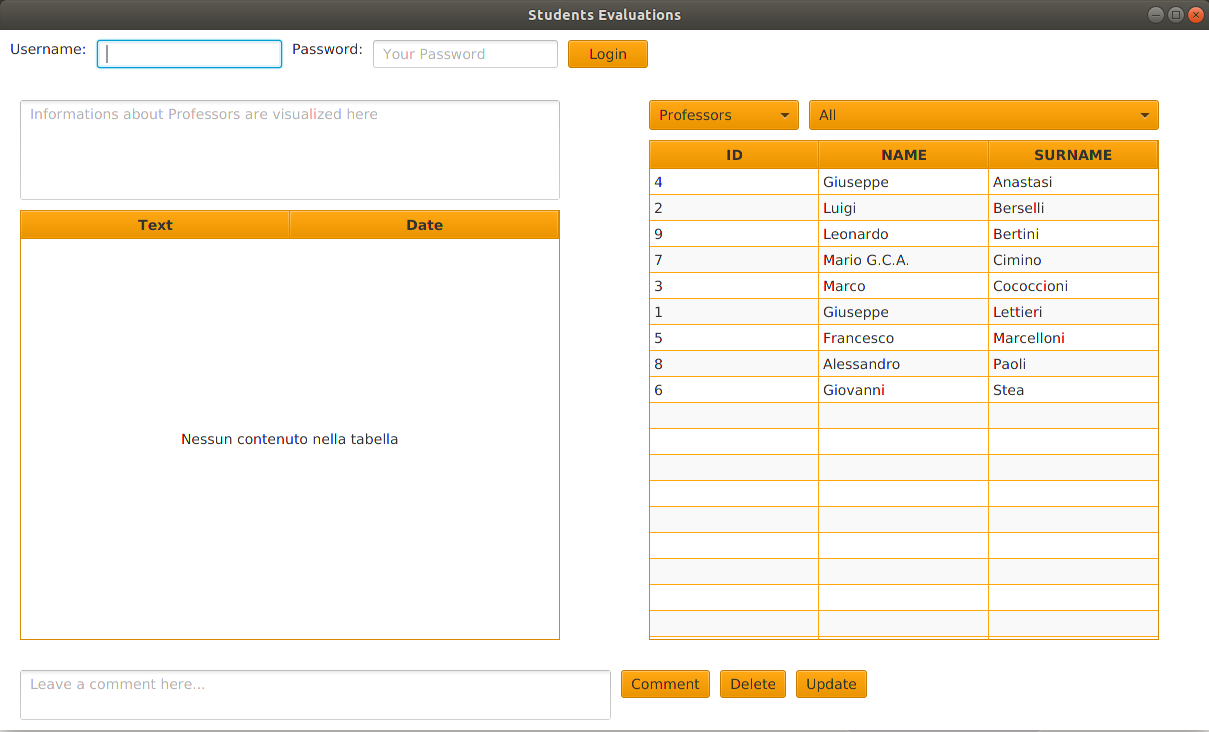
\includegraphics[width=0.7\textwidth]{./images/screens/screen0} 
\caption{Login page.}
\label{fig:screen0}
\end{figure}

\noindent In case you are not registered you can click the link at the bottom of the page to be redirected to a register page, figure~\ref{fig:screen1}, otherwise you can sign in the application and by default you get the interface shown in figure~\ref{fig:screen2}.
\begin{figure}[H]
\centering
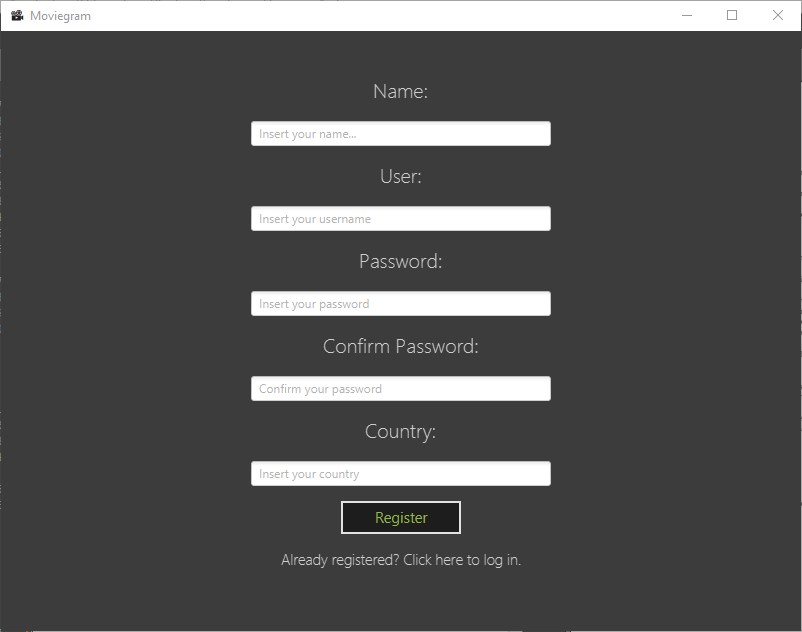
\includegraphics[width=0.7\textwidth]{./images/screens/screen1} 
\caption{Register page.}
\label{fig:screen1}
\end{figure}
\begin{figure}[H]
\centering
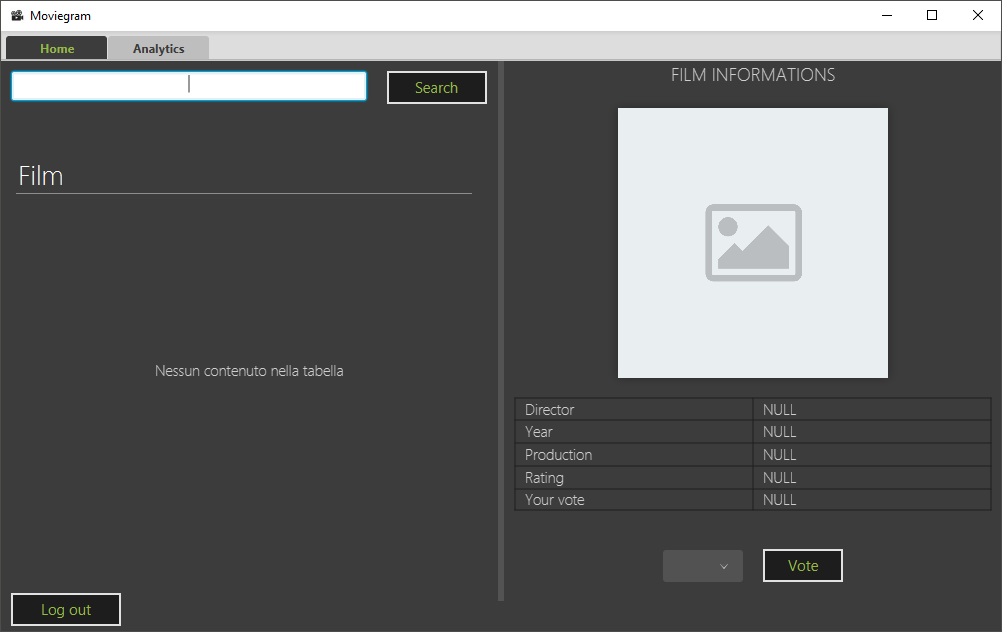
\includegraphics[width=0.7\textwidth]{./images/screens/screen2} 
\caption{Home page.}
\label{fig:screen2}
\end{figure}

\noindent From here you can search for a film by typing in the relative field and clicking the search button. You'll get a list of films that contains the text entered in the table below. Now you can select a film from the table and all the informations will be shown in the right pane of the application, figure~\ref{fig:screen3}. In the bottom right you are able to add a vote from 1 to 10 for the selected film.
\begin{figure}[H]
\centering
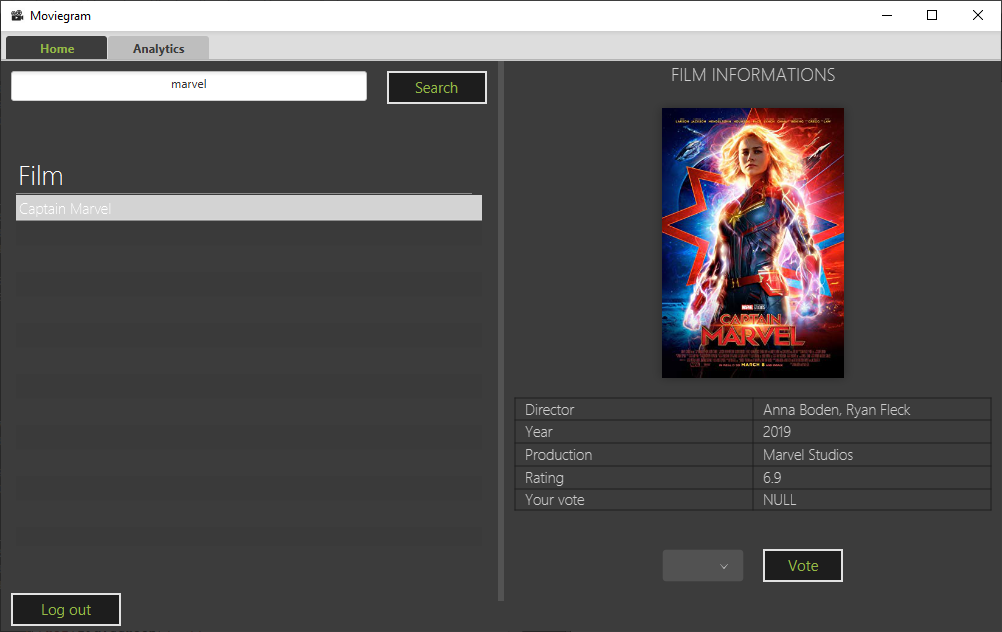
\includegraphics[width=0.7\textwidth]{./images/screens/screen3} 
\caption{Searching and selecting a film.}
\label{fig:screen3}
\end{figure}

\noindent In the top left of the page there are two tabs. by default after the login you are in the Home tab, by clicking the Analytics Tab you will see the following page.
\begin{figure}[H]
\centering
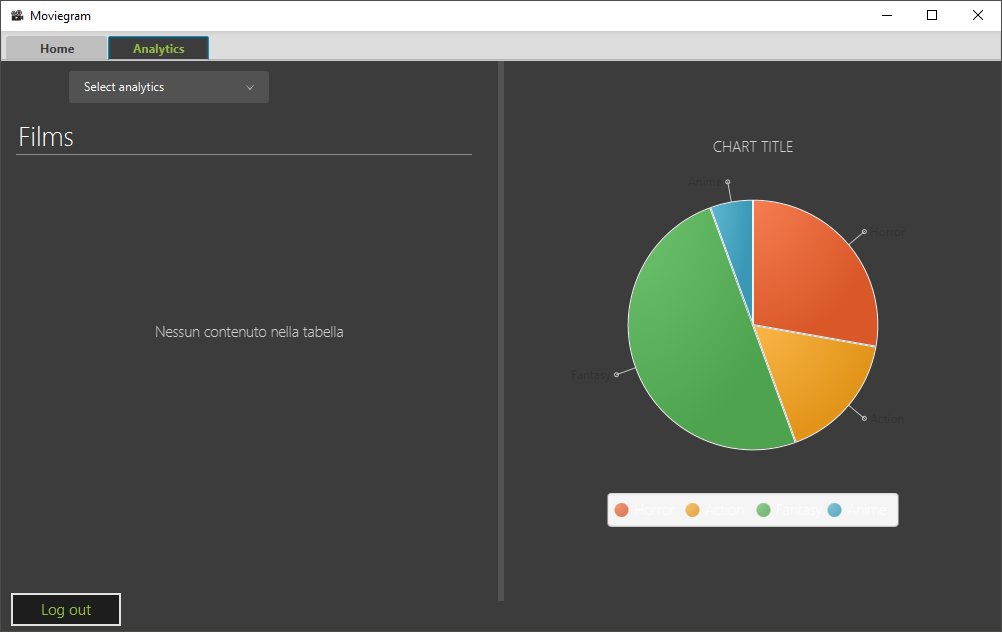
\includegraphics[width=0.7\textwidth]{./images/screens/screen4} 
\caption{Analytics page.}
\label{fig:screen4}
\end{figure}

\noindent Here you have a choice box (left) to select what kind of analytics you want to be performed from the existing ones, and another one to apply a filter (right). After selecting an analytics you will see the results in the table below, and for some of them you will get a piechart aswell, figure~\ref{fig:screen5}\\
\begin{figure}[H]
\centering
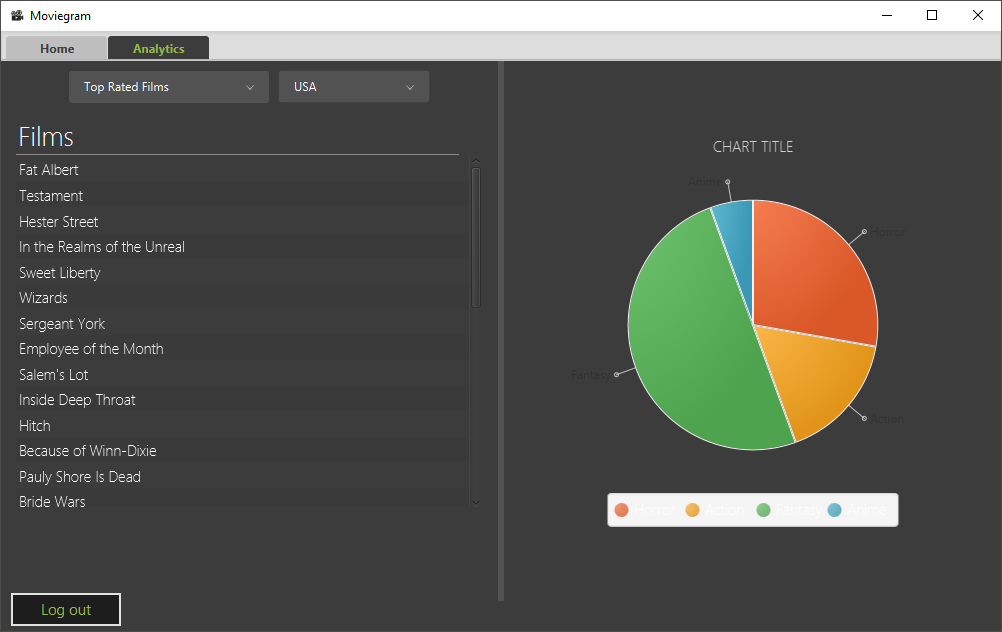
\includegraphics[width=0.7\textwidth]{./images/screens/screen5} 
\caption{Performing an analytics.}
\label{fig:screen5}
\end{figure}

\noindent To log out, just click on the appropriate button at the bottom.

\clearpage
%ADIMN MANUAL%
\subsection{Admin Manual}
If you have an admin user, you are entitled to make changes on the film lists. You need to log in inserting your username and password, and the application will recognize you as the administrator and show up a third tab called "Admin", figure~\ref{fig:admin0}
\begin{figure}[H]
\centering
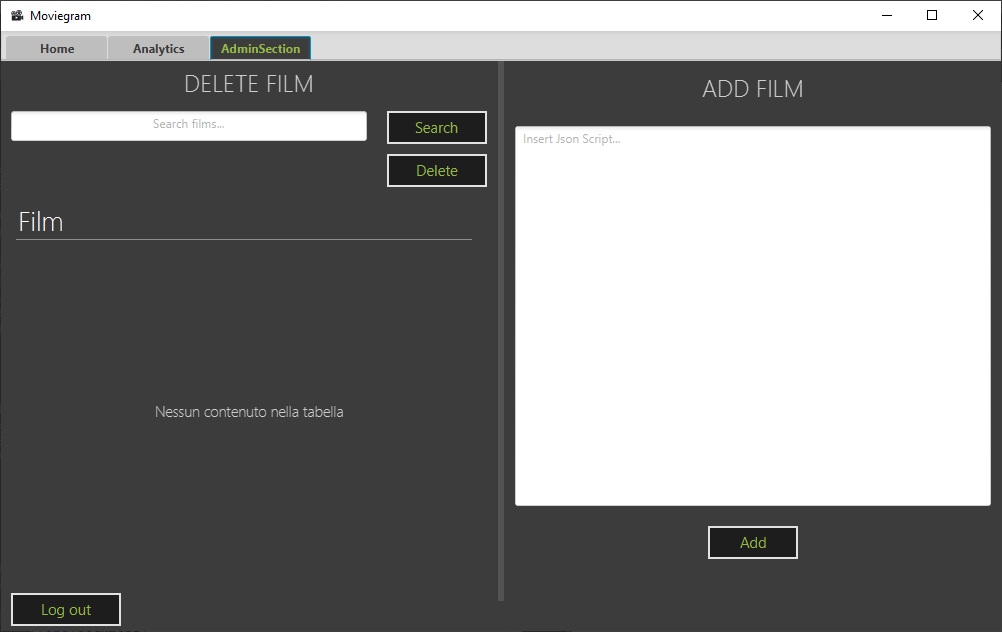
\includegraphics[width=0.7\textwidth]{./images/screens/admin0} 
\caption{Adnim page.}
\label{fig:admin0}
\end{figure}

\noindent In the Admin tab you can search for a film the same way the user did in the Home tab and after selecting one you are able to delete it by clicking the "Delete" button. On the right pane you are able to insert a json document in the text field, that represent a film in the database, and by clicking the Add button you will insert one or more films in the database (fig.~\ref{fig:admin1}).
\begin{figure}[H]
\centering
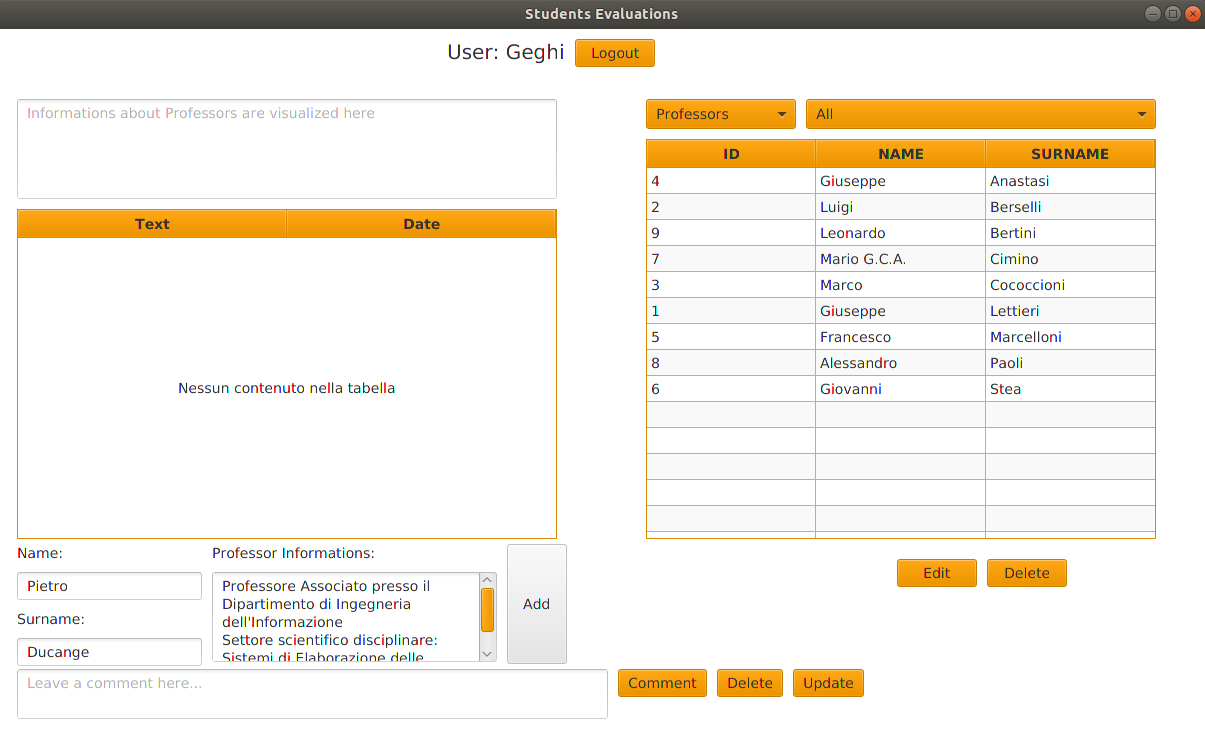
\includegraphics[width=0.7\textwidth]{./images/screens/admin1} 
\caption{Admin page after searching for a film.}
\label{fig:admin1}
\end{figure}

\end{document}
